\documentclass[dvisvgm,tikz]{standalone}
\begin{document}
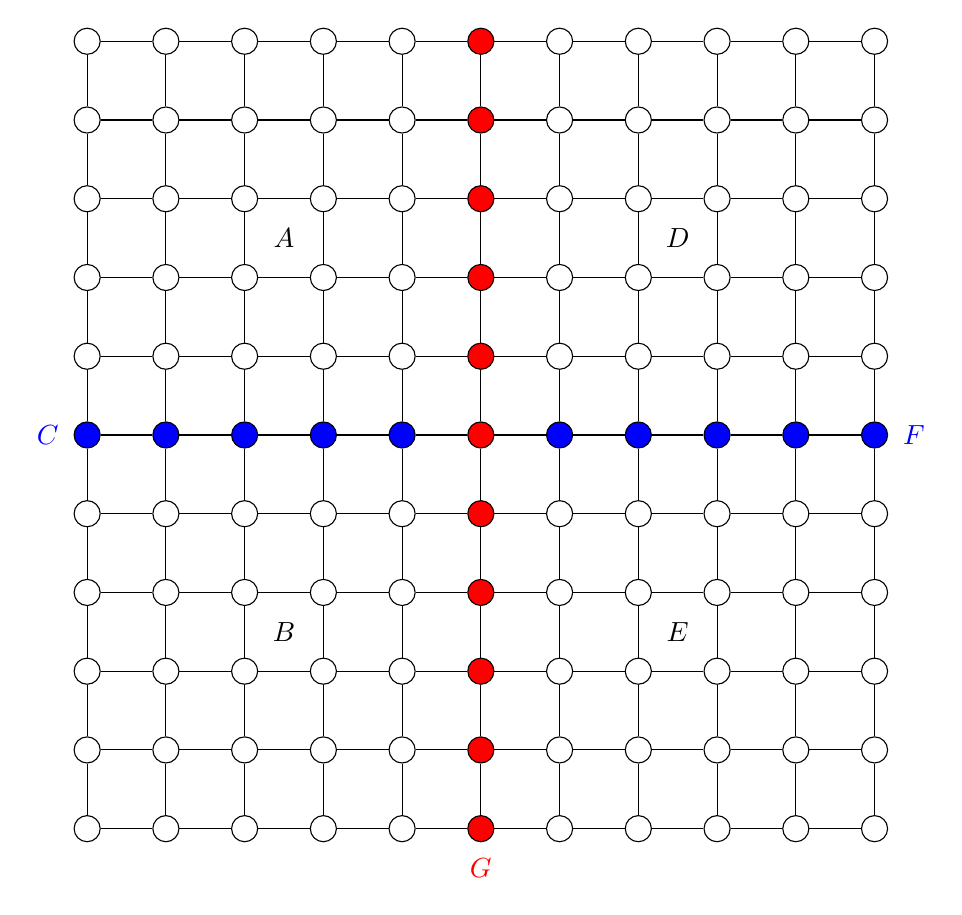
\begin{tikzpicture}

\foreach \x in {0,...,10}
  \foreach \y in {0,...,10} {
    \pgfmathparse{(\x==5) ? "red" : (\y == 5 ? "blue" : "white")}
    \edef\color{\pgfmathresult}
    \node[circle,draw,fill=\color] (\x\y) at (1.0+1.0*\x,1.0+1.0*\y) {};
  }

\foreach \x in {0,...,10}
  \foreach \y [count=\yi] in {0,...,9}
    \draw (\x\y)--(\x\yi) (\y\x)--(\yi\x);

\node at (3.5,8.5) {$A$};
\node at (3.5,3.5) {$B$};
\node at (8.5,8.5) {$D$};
\node at (8.5,3.5) {$E$};
\node at (0.5,6.0) {${\color{blue}C}$};
\node at (11.5,6.0) {${\color{blue}F}$};
\node at (6.0,0.5) {${\color{red}G}$};
  
\end{tikzpicture}
\end{document}
